% Besprechung 2019-11-14
\begin{enumerate}[label={Aufgabe H\arabic*},start=15]
	\item 
		\begin{enumerate}
			\item Bei der 5-Zustands-Prozessmodell gibt es 2 Zustände "Ready" und "Blocked" statt nur eines Zustands "Not Running" bei der 2-Zustands-Prozessmodell für Prozessen, die (noch) nicht ausgeführt sind. 

			Ein blockierter Prozess ist blockiert, weil er auf ein Ereignis wartet. Deswegen kann ein blockierter Prozess vor dem Eintreten des Ereignis gar nichts machen. Mithilfe dieser 2 getrennten Zustände kann man unterscheiden, ob eine Prozess rechenbereit sind ("Ready") oder nicht ("Blocked"). Damit arbeitet das CPU nur mit Prozesse, die rechenbereit sind. Das Aufhalten der Queue wegen Prozessen, die nichts machen können, wird vermeiden. Alles wird dann effizienter. 

			% New: 		Prozess wurde erzeugt, aber noch nicht zur Menge der ausführbaren Prozesse hinzugefügt
			% Blocked: 	Prozess wartet auf ein Ereignis, kann erst ...
			% Ready anstatt not running: Der Zustand erföllt im 2- und 5- Zustand Modell den selben Zweck. Wurde zur besseren Unterscheidung vom Blocked-Zustand Ready umbenannt..
			% Exit:		Pzess wurde durch das Betriebsystem aus der Menge der ausführbaren Prozesse enttfernt.

			\item Mit diesen 2 Zustände kann man 2 verschiedene Queues haben: ein "Ready" Queue und ein "Blocked" Queue. Ein Prozess, der blockiert ist, wird dann in das "Blocked" Queue geschickt. Als der Prozess wieder rechenbereit ist (z. B. durch das Eintreten eines Ereignisses), wird er dann in das "Ready" Queue geschickt. 

			Ein Vorteil davon ist, dass rechenbereite Prozesse von blockierten Prozessen wegen der getrennten Warteschlange nicht verhungert werden.

			Ein Nachteil davon ist, dass Prozesse nicht alle auf einer Warteschlange gestellt werden können. Das bedeutet mehr Overhead bei der Realisierung der Prozessverwaltung.

			% Je mehr Zustände enthalten sind, desto mehr Informationen liegen ber den Prozesse vor. ...

			% Vorteil: 	Das Suchen von Prozessen kann durch entsprechende Queues performanter gemacht werden.s
			% Nachteil: Komplexere Prozessinformationsverwalttung. Mehr benötigter Speicherplatz, etc.

			\item Scheduling bedeutet der Prozess, in dem das Scheduler einen rechenbereiten (bzw. im Zustand "Ready") Prozess wählt und gleichzeitig den aktuell abgearbeiteten Prozess unterbrecht bzw. beengidt.

			Dispatching bedeutet der Prozess, in dem der eigentlichen Kontextwechsel realisiert wird. Der Scheduler teilt dem Dispatcher die Information mit, welcher Prozess als nächster abgearbeitet werden soll. 

			% Scheduling Logische Einheit, die Auswahl desjenigen Prozessesm der als nächstes vom Ready
			% Dispatching_ Die tatsächeliche DDurchführung der Prozesszuteilung.
		\end{enumerate}
		\pagebreak
	\item 
		\begin{enumerate}
			\item \blanko

				\begin{center}
					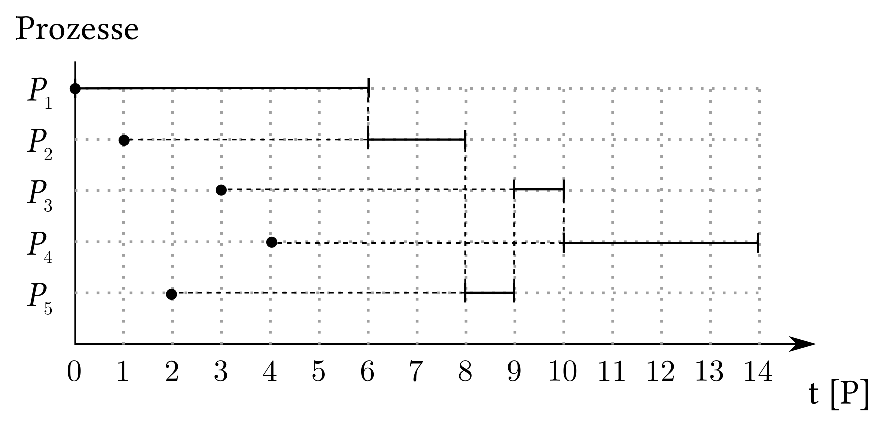
\includegraphics[width=0.7\textwidth]{16a.eps}
				\end{center}
			\item \blanko

				\begin{center}
					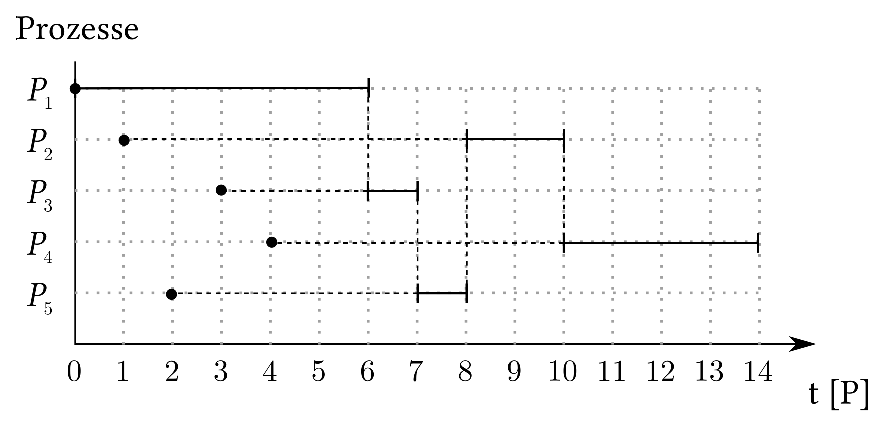
\includegraphics[width=0.7\textwidth]{16b.eps}
				\end{center}
			\item \textbf{FCFS}
				\vspace{1em}
				\begin{center}
					\renewcommand*{\arraystretch}{1.2}
					\begin{tabular}{@{}lllllll@{}}
						\toprule
						{\small Proz.} & {\small Ankunftz.} & {\small Bedienz.} & {\small Beendigungsz.} & {\small Verweildauer} & {\small Wartezeit} \\
						\midrule
						$P_1$ & $0$ & $6$ & $6$ & $6$ & $0$ \\
						$P_2$ & $1$ & $2$ & $8$ & $7$ & $5$ \\
						$P_3$ & $3$ & $1$ & $10$ & $7$ & $6$ \\
						$P_4$ & $4$ & $4$ & $14$ & $10$ & $6$ \\
						$P_5$ & $2$ & $1$ & $9$ & $7$ & $6$ \\
						\bottomrule
					\end{tabular}
				\end{center}
				\vspace{1em}

				Mittlere Verweildauer $ = (6+7+7+7+10)/5 = 7,4$ \\
				Mittlere Wartezeit $ = (0+5+6+6+6)/5 = 4,6$

				\pagebreak 
				\textbf{SJF}
				\vspace{1em}
				\begin{center}
					\renewcommand*{\arraystretch}{1.2}
					\begin{tabular}{@{}lllllll@{}}
						\toprule
						{\small Proz.} & {\small Ankunftz.} & {\small Bedienz.} & {\small Beendigungsz.} & {\small Verweildauer} & {\small Wartezeit} \\
						\midrule
						$P_1$ & $0$ & $6$ & $6$ & $6$ & $0$ \\
						$P_2$ & $1$ & $2$ & $10$ & $9$ & $7$ \\
						$P_3$ & $3$ & $1$ & $7$ & $4$ & $3$ \\
						$P_4$ & $4$ & $4$ & $14$ & $10$ & $6$ \\
						$P_5$ & $2$ & $1$ & $8$ & $6$ & $5$ \\
						\bottomrule
					\end{tabular}
				\end{center}
				\vspace{1em}

				Mittlere Verweildauer $ = (6+9+4+10+6)/5 = 7,0$ \\
				Mittlere Wartezeit $ = (0+7+3+6+5)/5 = 4,2$

		\end{enumerate}
		\vspace{1.5em}
	\item Sehen Sie bitte \texttt{u03-h17.txt}
\end{enumerate}